\documentclass[english, ing, kiv, he, iso690alph, pdf, viewonly]{fasthesis}
\title{Computer Vision Applications in~Video Recordings for Traffic Signal Detection and Classification on Czech Railways}
%\worktypespec{Technická zpráva}% <== this command is only applicable if 'oth' switch is used above
\author{Daniel}{Schnurpfeil}{Bc.}{}
\supervisor{Ing. Pavel Mautner, Ph.D.}
\stagworkid{12345}% <== the unique identifier of the work in the STAG information system
% \auxfrontmattercontent{% <== this command only makes sense if 'oth' switch is used above
	% \section*{Upozornění}%
	% Tento text bude vložen do front matteru\dots
% }


\assignment{zadani.pdf}


\signdate{}{}{}{V Plzni}% <== the longest local name in the Czech Rep.

\addbibresource{main.bib}% <== the file with the bibliographical database to be used throughout the text
% _____________________________________________________________________________
%
%
%	     DOCUMENT FRONTMATTER TEXTS
%
% _____________________________________________________________________________
%
\abstract{English abstract }{Czech abstract }
\keywords{computer vision, czech railways}
% _____________________________________________________________________________
%
%        ACKNOWLEDGEMENT
% _____________________________________________________________________________
%
\acknowledgement{}
% _____________________________________________________________________________
%
%        ADDITIONAL FRONT MATTER CONTENT
% _____________________________________________________________________________
% \auxfrontmattercontent{%
% \section*{Note for English readers}
% \fbox{\parbox[t]{\textwidth}{\textbf{%
% In case that your command of the Czech language is not sufficient for a perfect understanding of the whole of this document, please be so kind and open the file \filename"manual_en.pdf" which contains the same text (i.e. the user's manual for the \LaTeX{} template \filename"fasthesis.cls") in English.
% }}}}
% _____________________________________________________________________________
%
%
%	     DOCUMENT TEXT BEGINNING
%
% _____________________________________________________________________________
%
\begin{document}
\frontpages[tm] % or notm if the `trademark' declaration is not needed
\tableofcontents
% 
% -x---- ADDITIONAL COLOUR DEFINITIONS ----------------------------------------
%
\makeatletter%
\ifx\FASThesis@style\c@fullcolor%
	\definecolor{fascolor}{cmyk}{0.06, 0.27, 1.0, 0.12}%
	\definecolor{fascolordk}{cmyk}{0.05, 0.28, 1.0, 0.24}%
\else%
	\definecolor{fascolor}{cmyk}{0, 0, 0, 0.6}%
	\definecolor{fascolordk}{cmyk}{0, 0, 0, 0.75}%
\fi%
\makeatother%
\lstdefinestyle{plainsrc}{
	backgroundcolor=\color{fascolor!10},
	basicstyle=\ttfamily\footnotesize,
	numberstyle=\tiny\color{fascolordk},
	numbers=left,
	numbersep=5pt,
	keepspaces=true,
	tabsize=2,
	extendedchars=true,
	literate={á}{{\'a}}1 {č}{{\v{c}}}1 {ď}{{\v{d}}}1 {é}{{\'e}}1 {ě}{{\v{e}}}1 {è}{{\`{e}}}1 {í}{{\'{\i}}}1 {ľ}{{\v{l}}}1 {ň}{{\v{n}}}1 {ó}{{\'o}}1 {ŕ}{{\'r}}1 {ř}{{\v{r}}}1 {š}{{\v{s}}}1 {ť}{{\v{t}}}1 {ú}{{\'u}}1 {ů}{{\r{u}}}1 {ý}{{\'y}}1 {ž}{{\v{z}}}1
	{Á}{{\'A}}1 {Č}{{\v{C}}}1 {Ď}{{\v{D}}}1 {É}{{\'E}}1 {Ě}{{\v{E}}}1 {È}{{\`{E}}}1 {Í}{{\'I}}1 {Ľ}{{\v{L}}}1 {Ň}{{\v{N}}}1 {Ó}{{\'O}}1 {Ŕ}{{\'R}}1 {Ř}{{\v{R}}}1 {Š}{{\v{S}}}1 {Ť}{{\v{T}}}1 {Ú}{{\'U}}1 {Ů}{{\r{U}}}1 {Ý}{{\'Y}}1 {Ž}{{\v{Z}}}1
}
% -x---- END OF ADDITIONAL COLOUR DEFINITIONS ---------------------------------
% _____________________________________________________________________________
%
%
%        CHAPTER
%
% _____________________________________________________________________________
%
\chapter{Introduction}


Background on Railway Signaling Systems




Thesis objectives and scope


\chapter{Czech Railways}

todo - tady krátké intro

todo - zmínit evropský zabezpečovací systém, siemens mobility ...


\section{Situation in Recent Years}
todo - tady popsat situaci v čechách a na moravě (slezku)
\\
todo - zmínit - Dopravní a návěstní předpis pro tratě nevybavené evropským
vlakovým zabezpečovačem a že to je hlavní zaměření


\begin{figure}[!ht]

    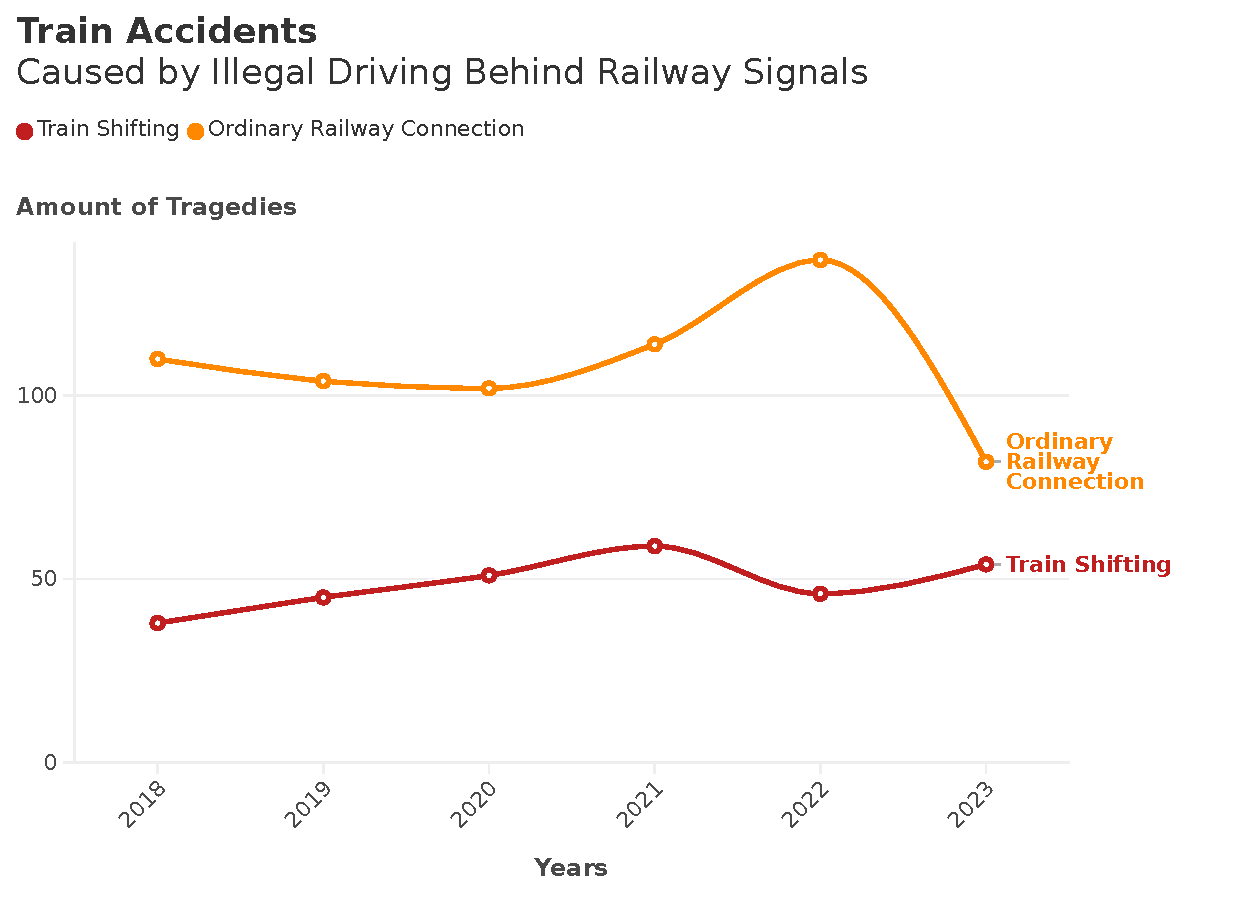
\includegraphics[width=1\linewidth]{Train Accidents.pdf}
    \caption{Train Accidents Caused by Illegal Driving Behind Railway Signals}
    \label{fig:enter-label}
\end{figure}


\section{Railway Signals}
% Visual characteristics and distinctions of different signals
Railway signals represent a visual communication tool for train drivers. Their main purpose is to show important safety information for train driver. These signals contain specific combinations of lights, shapes, and colors to transmit clear instructions about speed limits, track availability, and required actions. 

Light signals on Czech railways operate through a system of colored lights mounted on standardized signal posts. The most frequent signal colors are red, green, yellow, and white, with each color that carry distinct meaning. Red lights typically indicate stop request, while green lights could allow unlimited movement. The yellow light serves as a warning sign, preparing drivers for the following limitations. White lights are often in shunting\footnote{Shunting in railways is the process of moving trains, wagons within a station to assemble, disassemble, or relocate them for operational purposes.} signals or as additional indicators. 


The signals combine these colors in various patterns to communicate more complex messages. For example, two vertically positioned yellow lights (Figure \ref{fig:twice_yellow}) inform the driver to reduce speed and expect a stop signal ahead. The position and blinking of light(s) adds another piece of information to the basic colors. 
\begin{figure}[!ht]
    \centering
    
\includegraphics[width=0.1\linewidth]{myimgs/twice_yellow.pdf}
    \caption{Limit 40 km/h and warning}
    \label{fig:twice_yellow}
\end{figure}


Fixed railway signs complement the light-based system. These include physical signs and markers that display speed limits, distance warnings, and track identification. Their design emphasizes visibility in various weather conditions through reflective materials and high-contrast color schemes. Signal boards often use standardized shapes such as circles or white triangles that serve as warning signs. They are not part of the thesis. 

\newpage
\subsection{Single-Light Signals}
In this section we will, describe single-light signals and their characteristics.


The "Výstraha" signal allows the train to proceed but warns the driver to expect a "Stop" signal at the next main signal, which is placed at least the braking distance away. This signal is essential for preparing the driver for an upcoming stop, ensuring that the train can be safely halted if necessary.

The "Volno" signal indicates that the train can proceed without any speed restrictions. This signal is used on dependent main signals and pre-signals the next main signal, which will also display a permissive single-light signal. The "Volno" signal is crucial for maintaining smooth and efficient train operations, as it allows trains to continue at their maximum permitted speed.

Speed expectation signals, such as "Očekávejte rychlost 40 km/h," "Očekávejte rychlost 60 km/h," "Očekávejte rychlost 80 km/h," "Očekávejte rychlost 100 km/h," and "Očekávejte rychlost 120 km/h," inform the driver of the expected speed at the next main signal. These signals are placed at least the braking distance away from the next signal, ensuring that the driver has enough time to adjust the train's speed accordingly. The specific speed indicated by these signals can vary, with some signals indicating a range of possible speeds.

In cases where a rapidly flashing green light is accompanied by a yellow number, the number indicates the tens digit of the speed limit at the next main signal. This additional information helps the driver to anticipate the required speed adjustments, further enhancing the safety and efficiency of train operations.

Single-light signals play a vital role in the railway signaling system, providing clear and timely information to train drivers. Their design and placement are carefully considered to ensure that drivers can quickly and accurately respond to the signals, maintaining the safety and efficiency of railway operations.






\newpage
\subsection{Stop Signal (návěst Stůj)}

todo - tady popsat, info ze zdroje - ./czech-railway-trafic-lights-detection/

resources/

text\_resources/Výtah světelných návěstidel červená.pdf 




\newpage
\subsection{Multiple-Light Signals}
todo - tady popsat, info ze zdroje - ./czech-railway-trafic-lights-detection/

resources/

text\_resources/Výtah světelných návěstidel ostatni.pdf 



\newpage
\subsection{Foresignals (Předvěsti)}
todo - tady popsat, info ze zdroje - ./czech-railway-trafic-lights-detection/

resources/

text\_resources/Výtah světelných návěstidel predvesti.pdf 



\chapter{State of The Art}
this is related\cite{Staino2022}



\chapter{Data Analysis \& Methodology}

\section{Data Resources}

\newpage
\section{ETL}


Study of publicly available sources (e.g., YouTube channel parnici.cz)
Methods for extracting individual frames and image sequences ... \cite{lin2015microsoft}

\subsection{Data Annotation}
\subsubsection{YOLO}

\texttt{Limitations}


\subsubsection{Heuristics}


\subsubsection{Data Transformation}


\subsubsection{Datat Load}


\newpage
\section{ROI Detection}

Proposed methods for identifying light signals in images




\section{ROI Classification}
- enlarge bounding box (ROI) from yolo detections

\begin{figure}[!ht]
    \centering
    
\includegraphics[width=0.07\linewidth]{myimgs/example_roi.png}
    \caption{Original detection example (figure is from \cite{sprava_zeleznic_predpis})}
    \label{fig:original detection example}
\end{figure}


Techniques for recognizing specific signal aspects



% \subsection{Railway Detection}

% \subsection{Digits Detection}

% \subsection{Movement Detection}

\subsection{CNN Architecture Introduction}



\subsection{Yolo}





\chapter{Implementation}


Details of the implemented solution
\section{Dataset Storage}

\section{Experiment Playground}

\section{Training Scripts}


Technologies and libraries used
\section{Applied Technologies}

\subsection{Ultralytics Yolo}

\subsection{Open CV}

Challenges encountered and solutions applied
\subsection{Czech Metacenter}

\chapter{Results}

Description of the testing process


\section{Train Dataset}

\section{Eval Dataset}

\section{Test Dataset}
 parnici cz a strojvedouci .com

 
Process of compiling a comprehensive dataset for testing


Presentation of results


Analysis of system performance


\section{Signal Detection}

\subsubsection{Baseline}


\section{Signal Classification}


\subsubsection{Baseline}


\section{Signal Recognition}


Signal Detection


+


Signal Classification


\subsubsection{Baseline}


\chapter{Discussion}

Interpretation of results
Comparison with existing methods
Limitations of the current approach





\chapter{Conclusion}


%%%%%%%%%%%%%%%%%%%%%%%%%%%%%%%%%%%%%%%%%%%%%%%%%%%%%%%%%%%%%%%%%%%%%%%%%%%%%%%%%%%%%%%%%%



% create inspiration for section in my diploma thesis from following pdfs

% ...  in English ...  full title of the diploma thesis:   Computer Vision Applications in Video Recordings for Traffic Signal Detection and Classification on Czech Railways ...   note: don't use any GPT words and use American English on B2/C1 level ... \chapter{Railway signals and signs}
% ... content: Visual characteristics and distinctions of different signals ... don't write introduction ...

% use my language style .... here I provide for you some examples:
% The aim of the semester project is to learn how to implement a complex IR system
% using ready-made pre-processing libraries. A by-product will be a deeper under-
% standing of indexers, retrieval systems and lectures. When the assignment is clear, I can begin with possible solution proposals for im-
% plementation and then describe implementation details. The first thing to choose
% is a website to index. I have chosen the website which contains articles about data
% science. This website is for English speaking audience and it is part of medium.com
% portal, so the IR system can be extended by more topics than just data scinece. Due to personal preferences and by previous agreement there are two possible pro-
% gramming languages for implementation the IR system. First is Java and second
% is Python. I have chosen Python due to personal preferences to this program-
% ming language. The project implementation is suitable version 3.10 of Python
% interpreter. Usable dependencies are specified in the list bellow and were used for
% implementation. IR system is divided to several parts. The first part consists of scripts which are
% required to prepare indexed documents such as crawler or pre-processor. This part
% can be seen on the bottom of the Figure 1. The second part is web application
% based on Model View Controller (MVC) architecture. Both part are described in
% next sections. The crawler class is designed mainly for Towards Data Science website and pro-
% vides methods for sending ”polite” requests, extracting data from robots.txt file,
% article urls from sitemap.xml and also retrieving data from articles (<title> and
% <p>) html elements. Articles consist of index number, hash for detecting possible
% duplicates, dates when the articles were written, source URL, titles, authors,
% contents and website name For pre-processing is used nltk library with Porter Stemmer and English stop-
% words. Then I filtered common sentences at the beginning and the end of arti-
% cles. These common sentences does not carry any specific information. Thanks to
% Numpy library and some sort of invested time to optimization the pre-processing
% program can be faster than without using the Numpy library. Hierarchy of output
% data is similar to crawled contents, but it is in CSV format and Towards Data
% Science as page name is removed as common sentence. ... don't  write it implementation-focused but technical is okay, don't use too much bullet points

------------
generate Single-Light Signals section based on information:

Návěsti dovolující jízdu vlaku vyjádřené jedním světlem
(1) Návěsti dovolující jízdu vlaku vyjádřené jedním světlem dovolují strojvedoucímu jízdu vlaku
a na závislých hlavních návěstidlech (definice pojmu viz Čl. 111 tohoto předpisu) i předvěstí
návěst následujícího hlavního návěstidla.
(2) Návěsti vyjádřené jedním světlem strojvedoucímu vlaku přikazují jet nejvýše traťovou
rychlostí. Výjimkou jsou odjezdová (cestová) návěstidla při odjezdu jiným než přímým
směrem ve stanicích bez rychlostní návěstní soustavy a ve stanicích s nezávislými
návěstidly (definice pojmu viz Čl. 111 tohoto předpisu)
(3) Návěst Výstraha dovoluje jízdu vlaku a předvěstí návěst Stůj
na následujícím hlavním návěstidle, umístěném nejméně na zábrzdnou vzdálenost.
Obrázek 98
(4) Je li na vjezdovém (cestovém) návěstidle návěst Výstraha, strojvedoucí projíždějícího
vlaku jedná za vjezdu do stanice jako u vlaku pravidelně zastavujícího a musí ve stanici
s vlakem zastavit, pokud nejsou splněny podmínky tohoto předpisu pro odjezd vlaku.
135
SŽ D1 ČÁST PRVNÍ činnost od 1. července 2022
(5) Návěst Volno dovoluje jízdu vlaku a na závislém hlavním návěstidle
předvěstí dovolující návěst vyjádřenou jedním světlem na následujícím hlavním návěstidle.
Obrázek 99
(6) Je li projíždějící vlak zastaven u vjezdového (cestového) návěstidla stanice
s nezávislými návěstidly a vjezd je dovolován návěstí Volno, musí strojvedoucí
projíždějícího vlaku jednat za vjezdu do stanice jako u vlaku pravidelně zastavujícího
a musí ve stanici s vlakem zastavit, pokud nejsou splněny podmínky tohoto předpisu
pro odjezd vlaku.
(7) Návěst Očekávejte rychlost 40 km/h dovoluje jízdu
vlaku a předvěstí rychlost 40 km/h, 30 km/h nebo 50 km/h od následujícího hlavního
návěstidla, umístěného nejméně na zábrzdnou vzdálenost.
Obrázek 100
(8) Návěst Očekávejte rychlost 60 km/h dovoluje jízdu
vlaku a předvěstí rychlost 60 km/h nebo 70 km/h od následujícího hlavního návěstidla,
ve znění opravy č. 1 a změny č. 1 účinnost od 1. července 2024
umístěného nejméně na zábrzdnou vzdálenost.
Obrázek 101
(9) Návěst Očekávejte rychlost 80 km/h dovoluje jízdu
vlaku a předvěstí rychlost 80 km/h nebo 0 km/h od následujícího hlavního návěstidla,
umístěného nejméně na zábrzdnou vzdálenost.
Obrázek 102
SŽ D1 ČÁST PRVNÍ činnost od 1. července 2022
ve znění opravy č. 1 a změny č. účinnost od 1. července 2024
(10) Návěst Očekávejte rychlost 100 km/h dovoluje jízdu
vlaku a předvěstí rychlost 100 km/h nebo 0 km/h od následujícího hlavního návěstidla,
umístěného nejméně na zábrzdnou vzdálenost.
Obrázek 103
(11) Návěst Očekávejte rychlost 120 km/h
dovoluje jízdu vlaku a předvěstí rychlost 120 km/h od následujícího
hlavního návěstidla, umístěného nejméně na zábrzdnou vzdálenost.
Obrázek 104
(12) Je li nad rychle přerušovaným zeleným světlem hlavního návěstidla svítící žluté číslo
viz znázornění na obrázku 10 tohoto článku), je tím vyjádřena hodnota desetiny rychlosti
od následujícího hlavního návěstidla. Název návěsti se upravuje podle této rychlosti
(např. rychlost 120 km/h).

and use citations





Summary of achievements
Contributions to the field
Suggestions for future work


% _____________________________________________________________________________
%
%
%        BACK MATTER (BIBLIOGRAPHY, LISTS, ...)
%
% _____________________________________________________________________________
%
\backmatter
\printbibliography
\listoffigures
\listoftables
\listoflistings
% _____________________________________________________________________________
%
%		BACK COVER
% _____________________________________________________________________________
%
%\setbackpagepic{img/fav} % <== an example of one possible option (read this manual)
%\setqrcodebaseurl{https://mycloud.org/show=pdf&docid=} % <== another example
%\setbackpageqrcode{54321} % <== and one more (uncomment the one that makes sense for you)
\setbackpageqrcode
\backpage
\end{document}